%----------------------------------------------------------------------------------------
%    LA LLUM
%----------------------------------------------------------------------------------------
\section{La llum}
\subsection{Propietats de la llum}
\subsubsection*{Velocitat de la llum}
Els primers científics en intentar mesurar la velocitat de la llum han estat: Galileo Galilei (1638), Hippolyte Fizeau (1849), Michel Foucault (1850) i Albert Michelson (1880).
\begin{align}
    \boxed{c \equiv \SI{299792458}{\m\per\s}} \text{ (exactament)}.
\end{align}

\subsubsection*{Espectre electromagnètic}
\begin{figure}[H]
\centering
    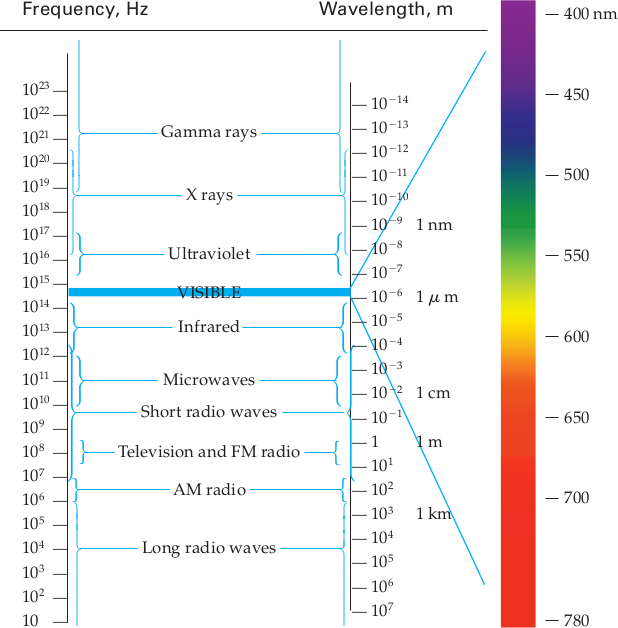
\includegraphics[width=0.8\textwidth]{images/3/31-espectre.png}
\caption{Espectre electromagnètic segons $\nu$ i $\lambda$.}
\end{figure}

\begin{figure}[H]
\centering
    WIP: GRAFIC BONIC 
\caption{Intensitat segons la font de llum}
\end{figure}

\subsubsection*{Dualitat ona--corpuscle}
Els fotons de llum estan quantitzats, de manera que $E$ només pot agafar valors que siguin múltiples enters de:
\begin{align}
    \boxed{E = h \nu = h \frac{v}{\lambda}}
\end{align}

on $h = \SI{6.626 e-34}{\J\s} = \SI{4.136 e-15}{\eV\s}$.

\subsubsection*{Interacció llum--matèria}
\begin{figure}[H]
\centering
    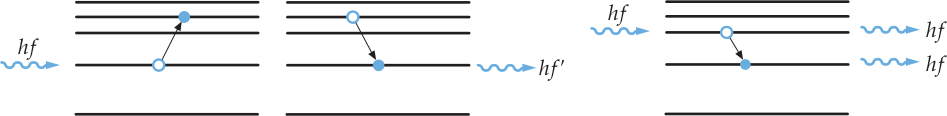
\includegraphics[width=\textwidth]{images/3/31-interaccio.png}
\caption{Processos d'absorció, emissió espontània i emissió estimulada, respectivament}
\end{figure}
\begin{itemize}
    \item Absorció de llum
    \item Emissió de llum
        \subitem Espontània
            \subsubitem Fluorescència: $\tau \sim \SI{10 e-8}{\s}$.
            \subsubitem Fosforescència: $\tau \uparrow \sim \si{\s}, \, \si{\minute}, \dots$
        \subitem Estimulada
\end{itemize}
%----------------------------------------------------------------------------------------
\subsection{Propagació de la llum}
\subsubsection*{Principi de Huygens}
Cada punt en un front d'ona primari actua com a font esfèrica secundària. La superposició d'aquests fronts d'ona secundaris és un nou front d'ona primari.
\begin{figure}[H]
\centering
    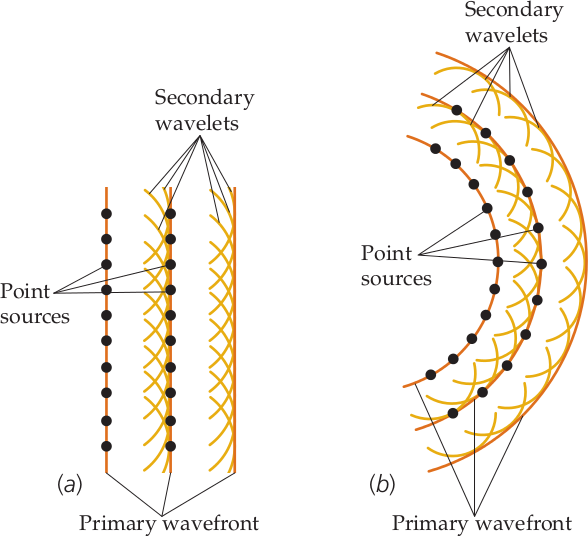
\includegraphics[width=0.6\textwidth]{images/3/32-huygens.png}
\caption{Construcció de Huygens dels fronts d'ona}
\end{figure}

\subsubsection*{Principi de Fermat}
 El camí fet per la llum entre dos punts és tal que el temps de recorregut del qual és mínim.

%----------------------------------------------------------------------------------------
\subsection{Reflexió i refracció}
\begin{figure}[H]
\centering
    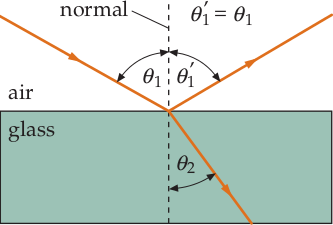
\includegraphics[width=0.5\textwidth]{images/3/33-refl-refr.png}
\caption{Diagrama de reflexió i refracció de la llum quan experimenta un canvi de medi}
\end{figure}
\subsubsection*{Llei de reflexió}
\begin{align}
    \boxed{\theta = \theta '}
\end{align}

\subsubsection*{Llei d'Snell de la refracció}
\begin{align}
    \boxed{n_{1} \sin \theta_{1} = n_{2} \sin \theta_{2}}
\end{align}
on $\begin{gathered} \boxed{n = \frac{c}{v}} \end{gathered}$ és l'índex de refracció de cada medi.

La refracció de la llum és una conseqüència del principi de Fermat.

\subsubsection*{Angle crític de reflexió total}
\begin{figure}[H]
\centering
    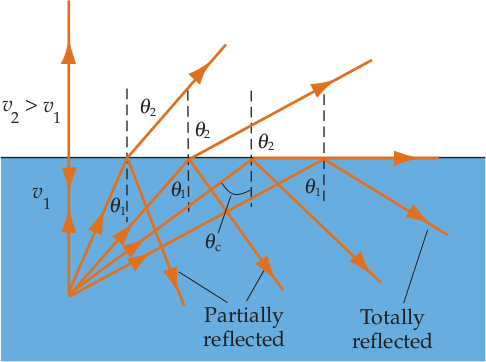
\includegraphics[width=0.6\textwidth]{images/3/33-angle-critic.png}
\caption{Diagrama d l'angle crític de reflexió total interna per a la refracció}
\end{figure}
\begin{align}
    n_{1} \sin \theta_{c} = n_{1} \sin \SI{90}{\degree} \Rightarrow \boxed{\sin \theta_{c} = \frac{n_{2}}{n_{1}}}
\end{align}

\subsubsection*{Casos concrets de refracció}

\subsection{Dispersió}
\subsubsection*{Tipus de superfícies}
\begin{itemize}
    \item Polida: actua com a una superfície especular.
        \begin{figure}[H]
        \centering
            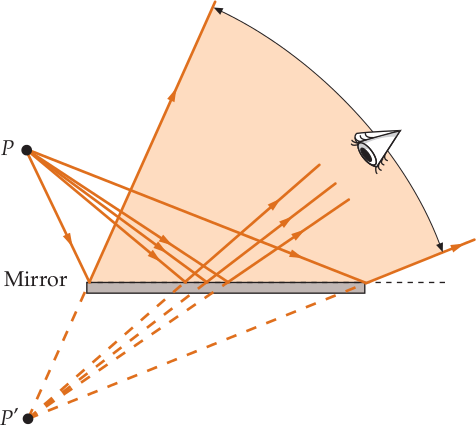
\includegraphics[width=0.4\textwidth]{images/3/34-especular.png}
        \caption{Superfície especular}
        \end{figure}
    \item No polida: actua com a una superfície difusora.
        \begin{figure}[H]
        \centering
            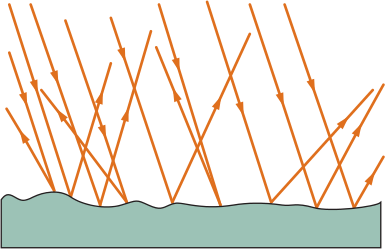
\includegraphics[width=0.4\textwidth]{images/3/34-difusor.png}
        \caption{Superfície difusora}
        \end{figure}
\end{itemize}

\subsubsection*{Dispersió cromàtica}
Com que la freqüència $\nu$ no varia en canviar la llum de medi, $n (\lambda) \Rightarrow$ cada color es refracta en una direcció diferent.
\begin{figure}[H]
\centering
    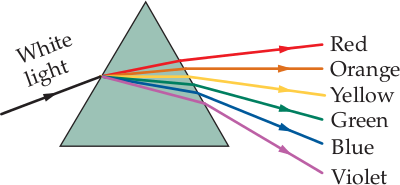
\includegraphics[width=0.6\textwidth]{images/3/34-disp-cromatica.png}
\caption{Dispersió cromàtica de la llum quan passa a través d'un prisma}
\end{figure}

%----------------------------------------------------------------------------------------
\subsection{Polarització de la llum}
En una ona electromagnètica, la direcció del camp elèctric és perpendicular a la direcció de propagació de la ona. Si el camp elèctric roman paral·lel a la direcció de propagació, es diu que l'ona està polaritzada linealment. Les ones produïdes per nombroses fonts no solen estar polaritzades, en aquests casos, el camp elèctric té components $x$ i $y$ que poden variar amb el temps.
\subsubsection*{Dicroisme (absorció selectiva)}

\subsubsection*{Reflexió selectiva}

\subsubsection*{Difusió Rayleigh}

\subsubsection*{Birefringència}